\documentclass{article}
\usepackage{amsmath}
\usepackage{amssymb}
\usepackage{parskip}
\usepackage{fullpage}
\usepackage{graphicx}
\usepackage{pgfplots}
\usepackage{neuralnetwork}
\usepackage{hyperref}
\usepackage{tikz}

\hypersetup{
    colorlinks=true,
    linkcolor=black,
    urlcolor=blue,
    pdftitle={Deep Learning},
    pdfpagemode=FullScreen,
}

\title{Deep Learning}
\author{Paolo Bettelini}
\date{}

\graphicspath{ {resources/} }

\begin{document}

\maketitle
\tableofcontents
\pagebreak

\section{Types of neurons}

\subsection{Brain neurons}

\begin{center}
    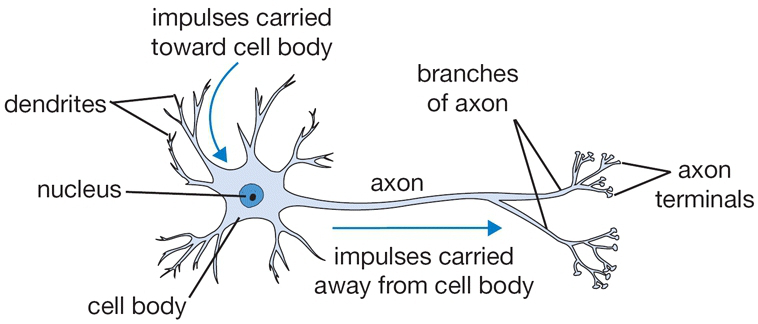
\includegraphics[scale=0.5]{neuron}
\end{center}

\subsection{Linear neurons}

% lecture 1.3

A linear neuron is very simple and computationally limited in what it can do.

\[
    y=b+\sum_{i} x_i w_i
\]

The output \(y\) is given by the bias \(b\) plus the sum of all the input connections \(x_i\) multiplied by their weight \(w_i\).

\subsection{Binary threshold neurons}

Binary threshold neurons output a \(1\) or a \(0\) depending on its weighted value.

Given a threshold \(\theta=-b\)
\begin{align*}    
    z&=b+\sum_{i} x_i w_i \\
    y&=\begin{cases}
        1 \text{ if } z\ge 0 \\
        0 \text{ otherwise}
    \end{cases}
\end{align*}

\subsection{Rectified Linear Neurons or Linear threshold neurons}

They compute a linear weighted sum of their inputs. \\
The output is a non-linear function of the total input.

Given a threshold \(\theta=-b\)
\begin{align*}    
    z&=b+\sum_{i} x_i w_i \\
    y&=\begin{cases}
        z \text{ if } z > 0 \\
        0 \text{ otherwise}
    \end{cases}
\end{align*}

\begin{center}
	\begin{tikzpicture}
		\begin{axis}[
            scale=0.75,
			xmin=-3,
			xmax=3,
			ymin=-3,
			ymax=3,
			xlabel={\(x\)},
			ylabel={\(y\)},
			scale only axis,
			axis lines=middle
		]
        \addplot[blue, ultra thick, domain=-3:0] {0};
        \addplot[blue, ultra thick, domain=0:2.5] {x};
		\end{axis}
	\end{tikzpicture}
\end{center}

\subsection{Sigmoid neurons}

They give a real-valued output that is a smooth and bounded function of their total input.

The logistic function is often used.

Given a threshold \(\theta=-b\)
\begin{align*}    
    z&=b+\sum_{i} x_i w_i \\
    y&=\frac{1}{1+e^{-z}}
\end{align*}

\begin{center}
	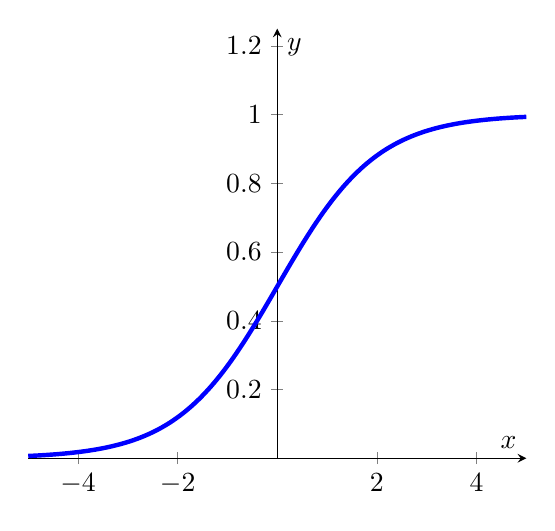
\begin{tikzpicture}
		\begin{axis}[
            scale=0.75,
			xmin=-5,
			xmax=5,
			ymin=0,
			ymax=1.25,
			xlabel={\(x\)},
			ylabel={\(y\)},
			scale only axis,
            smooth,
            samples=50,
			axis lines=middle
		]
        \addplot[blue, ultra thick, domain=-5:5] {1/(1+e^(-x))};
		\end{axis}
	\end{tikzpicture}
\end{center}

This function has smooth derivatives that change continuously. \\
This characteristic makes the learning process easier.

\pagebreak

% lecture 1.5

\section{Types of learning}

\subsection{Supervised learning}
Each training consists of making the network guess the target output \(t\) for a certain input \(x\), given the difference between the correct target and the guess we tweak the network.

There are two type of supervised learning

\subsubsection{Regression}
The target output is a numeric value of a vector of values. \\
To describe the error we can compute the square difference between the target output \(t\) and the actual output \(y\) of the module. \\
Often the value \(\frac{1}{2}{(t-y)}^2\) is used. The \(\frac{1}{2}\) coefficient is there to cancel the \(2\) out when differentiation is applied.

\subsubsection{Classification}
The target output is a class or label. Usually either \(1\) or \(0\).
There could also be multiple labels.
[\ldots]

\subsection{Reinforcement learning}
The output is an action of a sequence of actions to maximize the sum of rewards.

\subsection{Unsupervised learning}
[\ldots]

\pagebreak

% lecture 2.1

\section{Types of network architecture}

\subsection{Feed-forward neural network}

The most common type of neural network is the feed-forward neural network. \\
If there are more than one hidden layer it is called a \textit{deep} neural network.

\begin{center}
    \begin{neuralnetwork}[height=4]
        \inputlayer[count=3, bias=false, title=Input\\units]
        \hiddenlayer[count=4, bias=false, title=Hidden\\units] \linklayers{}
        \outputlayer[count=2, title=Output\\units] \linklayers{}
    \end{neuralnetwork}
\end{center}

At each layer there is a different representation of the initial input. \\
Similar things may become less similar and less similar things may become more similar.

In order to achieve this each layer must be a non-linear function of the activities in the previous layer.

\subsection{Recurrent network}

The same input might pass multiple times through the same neuron. \\
They are very difficult to train and more biologically realistic, hence they are more powerful.

Recurrent networks have the ability to remember information in their hidden state.

\subsection{Symmetrically connected network}

They are like recurrent network, but the connections between units are symmetrical
(they have the same weight in both directions).

Much easier to analyze than recurrent networks, but are more restricted in what they can do.

Symmetrically connected networks without hidden units are called \textit{Hopfield networks}.

% lecture 2.2

\pagebreak

\section{The perceptron}

A perceptron is an example of a statistical pattern recognition system. \\
The decision unit in a perceptron is a binary threadhold neuron.

\subsection{Learning biases}

We can learn the bias by treating it just like a regular weight,
rather than having a separate learning rule.
The bias is just the wight of an extra feature with the value of \(1\).

% Perceptron
\begin{center}
    \tikzset{basic/.style={draw,fill=none,text badly centered,minimum width=3em}}
    \tikzset{input/.style={basic,circle,minimum width=2.5em}}
    \tikzset{weights/.style={basic,rectangle,minimum width=2em}}
    \tikzset{functions/.style={basic,circle, minimum width=4em}}
    \begin{tikzpicture}[scale=1]
        % Draw input nodes
        \foreach \h [count=\hi ] in {$x_2$,$x_1$,$1$} {
            \node[input] (f\hi) at (0,\hi*1.25cm-1.5 cm) {\h};
        }
        % Dot dot dot ... x_n
        \node[below=0.62cm] (idots) at (f1) {\vdots};
        \node[input, below=0.62cm] (last_input) at (idots) {$x_n$};
        % Draw summation node
        \node[functions] (sum) at (4,0) {};
        % Draw arrows from input nodes to summation node
        \foreach \h [count=\hi ] in {$w_2$,$w_1$,$b$} {
            \path (f\hi) -- node[weights] (w\hi) {\h} (sum);
            \draw[->] (f\hi) -- (w\hi);
            \draw[->] (w\hi) -- (sum);
        }
        % Dot dot dot ... w_n
        \node[below=0.05cm] (wdots) at (w1) {\vdots};
        \node[weights, below=0.45cm] (last_weight) at (wdots) {$w_n$};
        % Add arrows for last node and last weight etc
        \path[draw,->] (last_input) -- (last_weight);
        \path[draw,->] (last_weight) -- (sum);
    
        % Labels
        \node[above=1cm]  at (f3) {inputs};
        \node[above=1cm] at (w3) {weights};
    \end{tikzpicture}
\end{center}

\subsection{Convergence procedure}

\begin{itemize}
    \item Add an extra component with value \(1\) to each input vector.
        This serves as the bias and is equivalent to the negative of the threshold.
    \item Pick training cases such that every training case will keep getting picked.
    \begin{itemize}
        \item If the output unit incorrectly outputs a \(0\), add the input vector to the weight vector.
        \item If the output unit incorrectly outputs a \(1\), subtract the input vector to the weight vector.
        \item If the output unit is correct, don't do anything.
    \end{itemize}
\end{itemize}

% lecture 2.3

\subsection{Geometric view}

Each training case defines a hyperplane (depending on the number of components) where
for an \textit{input vector} there is a \textit{weigth vector} that can be either on the
correct or wrong side of the hyperplane, depending on the resulting scalar product.
The plane goes through the origin and is perpendicular to the input vector.

Considering multiple training cases, the resulting vector shall be on all the good sides of all the hyperplanes.
Such point may not exist. However, if such point exists, the convergence procedure is guaranteed to find it.

% lecture 2.4

%\subsection{Proof of convergence}

%Here is the proof that the convergence procedure will get the right answer for all the training cases
%if such vector exists.

% lecture 2.5

\subsection{Convergence}

A region in the hyperspace where all the vectors in the regon satisfy all the training case exists if the dataset is linearly separable.
\\
This means that for example, considering a two-dimensional binary input vector, a perceptron cannot tell if the inputs are the same
(the XOR problem). This would lead to four inequalities that are impossible to satisfy.

\pagebreak

% lecture 3.1

\section{Linear neuron}

\subsection{Definition}

The perceptron learning procedure cannot extended to an arbitrary number of hidden layers. \\

The simplest example is a linear neuron with a squared error measure.
The goal is to minimize the errore over all training cases, rather than the weight vector to be in a given region.
The output of a linear neuron is a real value output which is a weighted sum of its input.

\[
    y=\sum_i w_i x_i
\]

For each training case we tweak each weight

\[
    \Delta w_i=\epsilon x_i(t-y)
\]

where \(\epsilon\) is some \textit{learning rate}, \(y\) is the guess of the network and \(t\) is the correct target output.

There is no guarantee with this kind of learning that the single weights will get better.

\subsection{The delta rule}

We can define the error of the network as the squared residuals summed over all training cases

\[
    E=\frac{1}{2} \sum_{n\in \text{traning}} {(t_n - y_n)}^2
\]

Now differentiate with respect to a single weight \(w_i\).
Note that \(E_n\) depends on \(y_n\) which depends on \(w_i\), so we can use the chain rule.
The purpose of the \(\frac{1}{2}\) term is to get a nice differentiation.

\begin{align*}
    \frac{\partial E}{\partial w_i}&=
    \frac{1}{2} \sum_n \frac{dE_n}{dy_n} \frac{\partial y_n}{\partial w_i} \\
    &= \frac{1}{2} \sum_n -2(t_n-y_n) x_{ni} \\
    &= - \sum_n (t_n-y_n) x_{ni}
\end{align*}

How the error changes as we change the weights, will be how the output changes as we change the weights
times how the error changes as the change the output.

So now the change of a weight is

\[
    \Delta w_i=-\epsilon \frac{\partial E}{\partial w_i} = \epsilon \sum_n x_{in}(t_n-y_n)
\]

% lecture 3.2

% lecture 3.3

\pagebreak

\section{Logistic neuron}

\subsection{Learning weights}

We can generalize the learning rule for a linear neuron to a logistic neuron, which is a non-linear neuron.
\\
\begin{align*}    
    z&=b+\sum_{i} x_i w_i \\
    y&=\frac{1}{1+e^{-z}}
\end{align*}

First we need to compute the derivatives of \(z\) with respect to the inputs \(x_i\), weights \(w_i\) and the output \(y\).

\[
    \frac{\partial z}{\partial w_i} = x_i,
    \quad
    \frac{\partial z}{\partial x_i} = w_i,
    \quad
    \frac{dy}{dz}=y(1-y)
\]

Now, using the chain rule, we can compute the derivative of the output with respect to \(w_i\)

\[
    \frac{\partial y}{\partial w_i}=\frac{dy}{dz}\frac{\partial z}{\partial w_i}=x_i y(1-y)
\]

Which means that the error \(E\) changes with respect to \(w_i\) as

\[
    \frac{\partial E}{\partial w_i} =
    \sum_n \frac{\partial E}{\partial y_n} \frac{\partial y_n}{\partial w_i} =
    -\sum_n x_{in} y_n (1-y_n)(t_n-y_n)
\]

Therefore the learning rule for a logistic neuron is

\[
    \Delta x_i = -\epsilon \frac{\partial E}{\partial w_i}=\epsilon \sum_n x_{in} y_n (1-y_n)(t_n-y_n)
\]

% lecture 3.4

\pagebreak

\section{Backpropagation}

So far we've learned how to learn the weights of a simple neural network (input units and output units).
However, we still lack the learning for more complicated neural nets with hidden layers.
This is because we don't know their features, in fact, they're called \textit{hidden units}
because we don't know what they ought to do.

One way to learn the weights would be to randomly modify a weight. If the network
gets better, keep the change, otherwise, discard it. This is, however, extremely
inefficient.

The backpropagation algorithm computes the gradient from the final layer to the first layer.

% https://brilliant.org/wiki/backpropagation/

\end{document}